%% 
%% Copyright 2007-2019 Elsevier Ltd
%% 
%% This file is part of the 'Elsarticle Bundle'.
%% ---------------------------------------------
%% 
%% It may be distributed under the conditions of the LaTeX Project Public
%% License, either version 1.2 of this license or (at your option) any
%% later version.  The latest version of this license is in
%%    http://www.latex-project.org/lppl.txt
%% and version 1.2 or later is part of all distributions of LaTeX
%% version 1999/12/01 or later.
%% 
%% The list of all files belonging to the 'Elsarticle Bundle' is
%% given in the file `manifest.txt'.
%% 

%% Template article for Elsevier's document class `elsarticle'
%% with numbered style bibliographic references
%% SP 2008/03/01
%%
%% 
%%
%% $Id: elsarticle-template-num.tex 168 2019-02-25 07:15:41Z apu.v $
%%
%%
%\documentclass[preprint, review, 12pt]{elsarticle}
\documentclass[preprint, 3p, times, twocolumn]{elsarticle}

%% Use the option review to obtain double line spacing
% \documentclass[authoryear,preprint,review,12pt]{elsarticle}

%% Use the options 1p,twocolumn; 3p; 3p,twocolumn; 5p; or 5p,twocolumn
%% for a journal layout:
%% \documentclass[final,1p,times]{elsarticle}
%% \documentclass[final,1p,times,twocolumn]{elsarticle}
%% \documentclass[final,3p,times]{elsarticle}
%% \documentclass[final,3p,times,twocolumn]{elsarticle}
%% \documentclass[final,5p,times]{elsarticle}
%% \documentclass[final,5p,times,twocolumn]{elsarticle}

%% For including figures, graphicx.sty has been loaded in
%% elsarticle.cls. If you prefer to use the old commands
%% please give \usepackage{epsfig}

%% The amssymb package provides various useful mathematical symbols
\usepackage{amssymb}
\usepackage{amsmath}
\usepackage{acronym}
\usepackage{algorithm}
\usepackage{algorithmic}
\usepackage{makecell}
\usepackage[inline]{enumitem}
\usepackage{bbm}
\usepackage[skip=2pt]{caption}
\usepackage{natbib}
\usepackage{xcolor}
\usepackage{booktabs}
\usepackage{hyperref}
\usepackage{rotating}
\usepackage{float}

%% The amsthm package provides extended theorem environments
%% \usepackage{amsthm}
\acrodef{RMSE}{root mean squared error}

%% The lineno packages adds line numbers. Start line numbering with
%% \begin{linenumbers}, end it with \end{linenumbers}. Or switch it on
%% for the whole article with \linenumbers.
%% \usepackage{lineno}
\journal{International Journal of Forecasting}

\begin{document}

\begin{frontmatter}

\title{Hierarchical Forecasting at Scale}

\author{}
% \author{%
%   Olivier~Sprangers \\
%   AIRLab, NL \\
%   University of Amsterdam, NL\\
%   \texttt{o.r.sprangers@uva.nl} \\
%   \And
%   Sebastian~Schelter \\
%   University of Amsterdam, NL \\
%   \texttt{s.schelter@uva.nl} \\
%   \And
%   Maarten~de~Rijke \\
%   University of Amsterdam, NL \\
%   \texttt{m.derijke@uva.nl} \\
% }



\begin{abstract}
  Hierarchical forecasting techniques allow creation of forecasts that are coherent with respect to a pre-specified hierarchy of the underlying time series. This targets a key problem in e-commerce, where we often find millions of products across many product hierarchies, and forecasts need to be made for both individual products and product aggregations. However, existing hierarchical forecasting techniques scale poorly when the number of time series increases, which limits their potential for application at a scale of millions of products. 
  
  In this paper, we investigate the use of learning a coherent forecast for millions of products with a single bottom-level forecast model by using a loss function that directly optimizes the hierarchical product structure. We implement our loss function using sparse linear algebra, such that the number of operations in our loss function scales quadratically rather than cubically with the number of products and levels in the hierarchical structure. The benefit of our sparse hierarchical loss function is that it provides practitioners a method of producing bottom-level forecasts that are coherent to any chosen hierarchy. In addition, removing the need for a post-processing step as used in traditional hierarchical forecasting techniques reduces the computational cost of the prediction phase in the forecasting pipeline. 
  
  In our tests on the public M5 dataset, our sparse hierarchical loss function performs up to 10\% better as compared to the baseline loss function. Next, we implemented our sparse hierarchical loss function within an existing gradient boosting-based forecasting model at bol.com, a large European e-commerce platform. Unfortunately, in this setting our sparse hierarchical loss resulted in a slightly worse forecasting performance as measured by RMSE of about 1\% at the product level, as compared to the the baseline model. 
  
\end{abstract}

\begin{keyword}
  Hierarchical forecasting, Large-scale forecasting, Efficiency in forecasting methods
\end{keyword}

\end{frontmatter}

\section{Introduction} \label{sec:intro}
In e-commerce, we are often faced with two forecasting challenges. First, forecasts at the lowest granularity - often the individual product level - are required but we also need forecasts for higher granularities, for example at the category, department or regional level. It is common that separate forecast models are made for each separate granularity, and as such these forecasts may not be coherent with each other. Hierarchical forecasting techniques \cite{hyndman_optimal_2011} aim to solve the problem of creating forecasts that are coherent with respect to a pre-specified cross-sectional hierarchy of the underlying time series. Second, contemporary large-scale forecasting applications require forecasting many time series concurrently \cite{bose_probabilistic_2017} and at increasingly lower time intervals, thus requiring faster training and prediction times, which in turn requires forecasting methods that scale better when the number of time series increases. In this work, we are interested in solving both these forecasting challenges.

\paragraph{Scaling challenges with existing hierarchical forecasting techniques} Reconciliation methods \cite{hyndman_optimal_2011,athanasopoulos_forecasting_2017,wickramasuriya_optimal_2019} apply a post-processing step that requires a matrix inversion that scales cubically with the number of products or product hierarchies. In settings with millions of products such as in e-commerce, this becomes computationally expensive at prediction time. Neural network methods \cite{rangapuram_endtoend_2021} directly optimize for the cross-sectional hierarchy in an end-to-end manner. However, these multivariate methods require a forward pass over all training samples at every training epoch, which becomes computionally expensive at training time in settings with millions of products. 
  
\paragraph{Sparse loss function} In order to overcome these scaling issues, we implement a sparse hierarchical loss function that directly optimizes the hierarchical structure. Our sparse implementation ensures that the number of operations in our loss function scales quadratically rather than cubically with the number of products and levels in the hierarchical structure, enabling computationally efficient training. The benefit of our sparse hierarchical loss function is that it provides practitioners a method of producing bottom-level forecasts that are coherent to any chosen hierarchy. In addition, removing the need for a post-processing step as used in traditional hierarchical forecasting techniques reduces the computational cost of the prediction phase in the forecasting pipeline.

\paragraph{Evaluation} We evaluate our sparse hierarchical loss function on a gradient-boosted forecasting system on the public M5 dataset \cite{makridakis_m5_2022} and a private dataset from our e-commerce partner. For the M5 dataset, we demonstrate that our implementation provides up to 10\% better forecasting performance as measured by RMSE compared with reconciliation methods and baseline bottom-level forecasting methods using a standard loss function. For the private dataset, we present the results of an offline test on the product-level forecast system of bol.com, a European e-commerce company with a catalog of millions of unnique products. Unfortunately, results from our offline test showed slightly worse performance as compared to the existing forecasting system at bol.com. [+ further explanation]

\paragraph{Contributions} In summary, the main contributions of this paper are:
\begin{enumerate}
  \item We present a sparse hierarchical loss function that enables direct end-to-end training of hierarchical forecasts in large-scale settings.
  \item We empirically demonstrate that a sparse hierarchical loss function can outperform existing hierarchical forecasting methods by up to 10\%.
  \item We show how are sparse hierarchical loss function scales to large-scale settings and demonstrate a reduction of prediction time of up to 4x compared to existing hierarchical forecasting reconciliation methods.
  \item [We present the results [and implementation details?] of an offline test of a forecasting system that forecasts millions of products daily at bol.com, a European e-commerce company.]]
\end{enumerate}

\section{Related work} \label{sec:relwork}

\paragraph{Forecasting for large-scale settings} Contemporary large-scale forecasting applications require forecasting many time series concurrently \cite{bose_probabilistic_2017}. In academia, there has been a surge in the use of neural network-based forecasting methods, which are methods that commonly learn a single forecast model that can produce forecasts for many time series. We refer the interested reader to the recent survey of \citet{benidis_deep_2023} for an overview of these methods. However, tree-based methods topped the M5 forecasting competition \cite{makridakis_m5_2022}, which is believed to be due to the strong implementations available of these algorithms \cite{januschowski_forecasting_2022}, such as the packages LightGBM \cite{ke_lightgbm_2017} or XGBoost \cite{chen_xgboost_2016}. Our own experience within bol.com confirms this view: the ease of use, execution speed and strong default performance are key reasons a tree-based method is often the default choice when creating a new forecast model.

\paragraph{Hierarchical forecasting} Hierarchical forecasting \cite{hyndman_optimal_2011, hyndman_fast_2016, taieb_coherent_2017, bentaieb_regularized_2019, wickramasuriya_optimal_2019} and temporal hierarchical forecasting techniques \cite{taieb_sparse_2017,athanasopoulos_forecasting_2017,rangapuram_coherent_2023,theodosiou_forecasting_2021} aim to solve the problem of creating forecasts that are coherent with respect to a pre-specified (temporal) hierarchy of the underlying time series. We divide hierarchical forecasting methods into \textit{Reconciliation methods} and \textit{Other methods}.

\textit{Reconciliation methods} These methods solve the hierarchical forecasting problem as a post-processing step by reconciling the forecasts to a pre-specified (temporal) hierarchy \cite{hyndman_optimal_2011, hyndman_fast_2016, taieb_coherent_2017, bentaieb_regularized_2019, wickramasuriya_optimal_2019, panagiotelis_forecast_2021}. Limitations of these approaches are (i) that they require a post-processing step, (ii) computing the reconciliation may be computationally expensive, as we show in Section~\ref{subsec:ourwork}, and (iii) approaches that are computationally less expensive tend to perform worse, as we show in Section~\ref{sec:experiments}. Recent work by \citet{taieb_sparse_2017, bentaieb_regularized_2019} has improved forecasting performance of previous reconciliation approaches but at the expense of even higher computational cost, as we explain in Section~\ref{sec:background}. \citet{zhang_optimal_2023} study the problem of reconciling hierarchical forecasts where some of the base forecasts are immutable, i.e. these are not allowed to be modified by the reconciliation method. However, this work also does not address the scalability issues we identify in Section~\ref{subsec:ourwork}.

\textit{Other methods} In \cite{rangapuram_endtoend_2021,rangapuram_coherent_2023} neural network-based end-to-end hierarchical probabilistic forecasting method are proposed to solve the hierarchical forecasting problem. More recently and most closely related to our work, \citet{han_simultaneously_2021} introduced SHARQ, a method that reconciles probabilistic hierarchical forecasts during training by employing a regularized loss function that enforces hierarchical consistency of bottom-up forecasts through regularization.

\section{Background} \label{sec:background}
Suppose we have a time series \(\vec{y}_t\), where \(t\) denotes the time stamp. We are interested in estimating future values \(\hat{y}_{t}\) of the time series by employing a model \(f\) based on past values \(y_{t-1}, \dots, y_{t-T}\) of the time series and additional attributes \(X\):
\begin{equation}
  \hat{y}_{t} = f(y_{t-1}, \dots, y_{t-T}, X_{t}, X_{t-1}, \dots, X_{t-T}).
\end{equation}
In our hierarchical forecasting setting, we aim to create forecasts for many time series concurrently, whilst adherring to pre-specified hierarchical relationships that exist between the time series. This can be formalized as \cite{hyndman_forecasting_2021}:
\begin{equation} \label{eq:hfp}
  \tilde{\textbf{y}}_{t} = SP\hat{\textbf{y}}_{t} \;,
\end{equation}
where \(\hat{\textbf{y}}_{t} \in \mathbb{R}^{m} \) denotes the vector of forecasts for all \(m\) time series in the hierarchy, \(S \in \{0, 1\}^{m \times n}\) is a matrix that defines the hierarchical relationship between the \(n\) bottom-level time series and the \(m^* = m - n\) aggregations, and \(P \in \mathbb{R}^{n \times m}\) is a matrix that encapsulates the contribution of each forecast to the final estimate. We can use the matrix \(P\) to define various forecast contribution scenarios. Note that we can straightforwardly extend Equation~\eqref{eq:hfp} to the setting of \textit{temporal hierarchies} \cite{athanasopoulos_forecasting_2017,rangapuram_coherent_2023} by considering forecasts of different time granularities in our vector of base forecasts \(\hat{\textbf{y}}_{t}\) and using an appropriate choice of \(S\) to aggregate series of a different time granularity.

The optimal solution to the problem in Equation~\eqref{eq:hfp} can be found using \textit{Reconciliation methods} and \textit{Other methods}.

\paragraph{Reconciliation methods}

\textit{MinTShrink} \cite{wickramasuriya_optimal_2019} and variants find the optimal \(P\) matrix by solving the following minimization problem for a particular choice of \(W\):
\begin{align}
  \min_P &(\hat{\textbf{y}}_{t} - SP\hat{\textbf{y}}_{t})^T W (\hat{\textbf{y}}_{t} - SP\hat{\textbf{y}}_{t}) \nonumber \\
  & \text{s.t.} \quad PS=I. \label{eq:minp}
\end{align}
Assuming \(W\) is positive definite, this has the following solution (ref. Theorem 1 of \cite{wickramasuriya_optimal_2019}):
\begin{align} 
  P &= (S^TW^{-1}S)^{-1}S^TW^{-1} \nonumber \\
    &= (J - JWU(U^TWU)^{-1}U^T) \;, \label{eq:p1}
\end{align}
in which \(S\) is partitioned as \(S^T = [C^T \; I_n]\), \(J = [0_{n \times m^*} \; I_n]\), \(U^T = [I_{m^*} \; -C]\). In \textit{MinTShrink}, \(W\) is estimated using the shrunk empirical covariance estimate of \cite{schafer_shrinkage_2005}. Simpler choices for \(W\), such as the identity matrix, reduce the solution to the \textit{Ordinary Least Squares (OLS)} solution of \cite{hyndman_optimal_2011}. In \textit{ERM}, \citet{bentaieb_regularized_2019} note than \textit{MinTShrink} and variants rely on the assumption of unbiasedness of the base forecasts. Therefore, they relax this assumption by formulating the hierarchical reconciliation problem as an \textit{Empirical Risk Minimization} problem, introducing the \textit{ERM} method. In addition, they propose two regularized variants of \textit{ERM} aimed at reducing forecast variance.

\paragraph{Other methods} \textit{Hier-E2E} \cite{rangapuram_endtoend_2021} solves the problem of Equation~\eqref{eq:hfp} by learning a neural network model that combines the forecasting and reconciliation step in a single model, resulting in an end-to-end solution removing the need for a post-processing step. Similarly, \textit{COPDeepVAR} \cite{rangapuram_coherent_2023} is an end-to-end neural network method that enforces temporal hierarchies, however this is a univariate method that is not able to enforce structural hierarchies (i.e. cross-sectional hierarchies) simultaneously, and therefore not suited to our task. \textit{SHARQ} \cite{han_simultaneously_2021} also moves the reconciliation step into the training phase and achieves reconciliation using a regularized loss function, where the regularization enforces the coherency. However, this method does not enforce absolute coherency to the hierarchy.

\subsection{Scaling issues of hierarchical forecasting methods} \label{subsec:ourwork}

Our main motivations of this paper are the limitations of prior work for problem settings with many time series.

\paragraph{Scaling issues with reconciliation methods} \label{sec:scalingissuesreconmethods}
In reconciliation methods, we see the following issues when scaling to many time series:
\begin{itemize}
  \item The reconciliation is performed as a \textit{post-processing} step, and thus has to be performed as an additional step after generating the base forecasts. Even though \(P\) in Eq.~\ref{eq:hfp} can be computed once using Eq.~\eqref{eq:p1}, the reconciliation still needs to be performed after each base forecast is produced. Also, \(P\) ideally is sparse \cite{bentaieb_regularized_2019}, but no reconciliation method guarantees this so computing Eq.~\ref{eq:hfp} will generally be a dense matrix-vector product that scales with the number of timeseries.
  \item For \textit{MinTShrink} \cite{wickramasuriya_optimal_2019}, estimating \(W\) according to the method of \cite{schafer_shrinkage_2005} is computationally expensive, as computing this estimate has a computational complexity of \(O(Nn^2)\), with \(N\) denoting the number of training samples used to compute the shrunk covariance estimate. In addition, the shrunk covariance estimate of \cite{schafer_shrinkage_2005} is not guaranteed to give consistent results in high-dimensional settings \cite{touloumis_nonparametric_2015}, making it less applicable for problem settings with many time series. Finally, the estimate for \(W\) will generally be a dense matrix, so we cannot make use of efficient sparse algorithms to solve Eq.~\eqref{eq:p1}. However, even for simpler, sparse choices of \(W\) (such as the identity matrix of \textit{OLS} \cite{hyndman_optimal_2011}), we still need to invert a matrix of size \(m^* \times m^*\) in order to solve Eq.~\eqref{eq:p1}, which becomes computationally costly for problems with many aggregations, which naturally arise in retail forecasting scenarios. For example, for the M5 retail forecasting competition \cite{makridakis_m5_2021}, \(m^*=12,350\), even though there are only 3,049 unique products in this dataset.  
  \item For \textit{ERM} and its regularized variants \cite{bentaieb_regularized_2019}, we need to either invert multiple dense matrices that scale quadratically with the number of time series, or we need to compute a Kronecker product that scales quadratically with the number of time series, followed by an expensive lasso search procedure. Improving the computational complexity of the \textit{ERM} methods is also mentioned in \cite{bentaieb_regularized_2019} as an avenue for future work.
\end{itemize}

\paragraph{Scaling issues with other methods} \label{sec:scalingissuesneuralmethods} \textit{Hier-E2E} \cite{rangapuram_endtoend_2021} is a multivariate method, which means both input and output of the neural network scale with the number of time series. For neural networks, this significantly adds to the training cost and parameter cost as a large amount of parameters are required to handle all the separate time series. This in turn requires GPUs with more memory to train these models, which increases cost to operate them. 

\section{Sparse Hierarchical Loss} \label{sec:sparsehloss}
We now present our main technical contribution. To find the best forecasts for the hierarchical forecasting problem \eqref{eq:hfp}, we try to find a model \(f(\cdot)\) by gradient-based optimization of the following loss function:
\begin{align} \label{eq:whloss}
  L &= \sum \left[ \frac{\frac{1}{2}(\textbf{y}_{t} - \hat{\textbf{y}}_{t})^2}{l \sum_{j=1}^n S_{ij}} \right] \; ,
\end{align}
in which \(l\) denotes the number of levels in the hierarchy and \(ij\) are the (row, column) indices of the elements of the \(S\)-matrix. Note that \eqref{eq:whloss} resembles the \textit{Weighted Root Mean Squared Error} from the M5 competition \cite{makridakis_m5_2022}.

We are interested in finding bottom-level forecasts that can be aggregated according to a pre-specified hierarchy \(S\), thus \(P = [0_{n \times m^*} \; I_n] \) in \eqref{eq:hfp} and:
\begin{equation} \label{eq:hfpbu}
  \tilde{\textbf{y}}_{t} = S \hat{\textbf{y}}^n_{t} \;,
\end{equation}
where \(\hat{\textbf{y}}^n_{t}\) denotes the vector of bottom-level forecasts of length \(n\). 
Considering only bottom-level forecasts has a number of benefits: (i) each forecast is coherent to any hierarchy by design, and (ii) we reduce the number of required forecasts from \(m\) to \(n\), which can be a significant reduction (there is no need for a forecast for \(m^*\) aggregations in the hierarchy). 
Now, we can derive the gradient and hessian of \eqref{eq:whloss} with respect to the bottom-level forecasts \(\hat{\textbf{y}}^n_{t}\) : 
\begin{align} 
  \frac{\partial L}{\partial \hat{\textbf{y}}_{t}} &=  \left[ \frac{(\hat{\textbf{y}}_{t} - \textbf{y}_{t})}{l \sum_{j=1}^n S_{j}} \right] \;, \label{eq:hfp_grad} \\
  \frac{\partial L}{\partial \hat{\textbf{y}}^n_{t}} &= \left(\frac{\partial L}{d \hat{\textbf{y}}_{t}}\right)^\intercal S \;, \label{eq:hfpbu_grad}  \\
  \frac{\partial^2 L}{\partial \hat{\textbf{y}}_{t}^{n, 2}} &= \left[ \sum_{j=1}^n \frac{S}{l \sum_{j=1}^n S_{ij}} \right]\;. \label{eq:hfpbu_hess}                                               
\end{align}

\paragraph{Analysis} The best possible forecast is achieved when the loss \eqref{eq:whloss} is minimized, or equivalently when the gradient \eqref{eq:hfp_grad} is zero:
\begin{align} 
  \frac{\partial L}{\partial \hat{\textbf{y}}_{t}} &=  \left[ \frac{(\hat{\textbf{y}}_{t} - \textbf{y}_{t})}{l \sum_{j=1}^n S_{j}} \right] \;, \nonumber \\
                                                   &=  \left[ \frac{(S \hat{\textbf{y}}^n_{t} - S \textbf{y}^n_{t})}{l \sum_{j=1}^n S_{j}} \right] \;, \nonumber \\
                                                   &=  \left[ \frac{S(\hat{\textbf{y}}^n_{t} - \textbf{y}^n_{t})}{l \sum_{j=1}^n S_{j}} \right] \;, \nonumber
\end{align}
which becomes zero when \(\hat{\textbf{y}}^n_{t} = \textbf{y}^n_{t}\). Thus, the best forecast model is found when each bottom-level forecast equals the ground truth. This is equivalent to the standard (i.e., non-hierarchical) squared error loss often used in forecasting problems. We argue that our hierarchical loss gradient can be seen as a \textit{smoothed} gradient compared to the standard squared error loss gradient (i.e. \((\hat{\textbf{y}}^n_{t} - \textbf{y}^n_{t})\)). For example, consider the canonical case where we have two bottom-level time series (\(n=2\)) and a single aggregation (the sum of the two time series), thus \(m^* = 1\) and \(m = m^* + n = 3\). Finally, there are two levels in our hierarchy, thus \(l = 2\). Now, we have:
\begin{align}
  \tilde{\textbf{y}}_{t} = \underbrace{
    \begin{bmatrix}
    1 &1 \\
    1 &0 \\
    0 &1
    \end{bmatrix}}_S 
    \underbrace{    
    \begin{bmatrix}
      \hat{\textbf{y}}^1_{t} \\
      \hat{\textbf{y}}^2_{t}
    \end{bmatrix}}_{\hat{\textbf{y}}^n_{t}} \;,
\end{align}
and the gradient of the loss with respect to the bottom level time series \eqref{eq:hfpbu_grad} reads:
\begin{align} 
  \begin{bmatrix}
  \frac{\partial L}{\partial \hat{\textbf{y}}^1_{t}} \\
  \frac{\partial L}{\partial \hat{\textbf{y}}^2_{t}}
  \end{bmatrix}^\intercal 
  &= \left[ \frac{S(\hat{\textbf{y}}^n_{t} - \textbf{y}^n_{t})}{l \sum_{j=1}^n S_{j}} \right]^\intercal S  \;, \nonumber \\
  &=  \left[ \frac{
    \begin{bmatrix}
      1 &1 \\
      1 &0 \\
      0 &1
    \end{bmatrix}
    \left(  
    \begin{bmatrix}
      \hat{\textbf{y}}^1_{t} \\
      \hat{\textbf{y}}^2_{t}
    \end{bmatrix}  
    - 
    \begin{bmatrix}
      \textbf{y}^1_{t} \\
      \textbf{y}^2_{t}
    \end{bmatrix}  
    \right)
    }{2 
    \begin{bmatrix}
      2 &1 &1
    \end{bmatrix}^\intercal  
    } \right]^\intercal
    \begin{bmatrix}
      1 &1 \\
      1 &0 \\
      0 &1
    \end{bmatrix}  \;, \nonumber \\
  &=  \left[ \frac{
    \begin{bmatrix}
      \hat{\textbf{y}}^1_{t} + \hat{\textbf{y}}^2_{t} - \textbf{y}^1_{t} - \textbf{y}^2_{t} \\
      \hat{\textbf{y}}^1_{t} - \textbf{y}^1_{t} \\
      \hat{\textbf{y}}^2_{t} - \textbf{y}^2_{t} \\
    \end{bmatrix}
    }{ 
    \begin{bmatrix}
      4 &2 &2
    \end{bmatrix}^\intercal  
    } \right]^\intercal
    \begin{bmatrix}
      1 &1 \\
      1 &0 \\
      0 &1
    \end{bmatrix}  \;, \nonumber \\
  &=          
   \begin{bmatrix}
     \frac{1}{4}(\hat{\textbf{y}}^1_{t} + \hat{\textbf{y}}^2_{t} - \textbf{y}^1_{t} - \textbf{y}^2_{t}) \\
     \frac{1}{2}(\hat{\textbf{y}}^1_{t} - \textbf{y}^1_{t}) \\
     \frac{1}{2}(\hat{\textbf{y}}^2_{t} - \textbf{y}^2_{t}) \\
   \end{bmatrix}^\intercal
   \begin{bmatrix}
     1 &1 \\
     1 &0 \\
     0 &1
   \end{bmatrix}  \;, \nonumber \\
  &=
  \begin{bmatrix}
    \frac{3}{4}(\hat{\textbf{y}}^1_{t} - \textbf{y}^1_{t}) + \frac{1}{4}(\hat{\textbf{y}}^2_{t} - \textbf{y}^2_{t}) \\
    \frac{1}{4}(\hat{\textbf{y}}^1_{t} - \textbf{y}^1_{t}) + \frac{3}{4}(\hat{\textbf{y}}^2_{t} - \textbf{y}^2_{t}) \\
  \end{bmatrix}^\intercal  \; \nonumber.      
\end{align}  
Hence, we \textit{smooth} the bottom-level gradient by adding to it portions of the gradients of all aggregations the bottom-level series belongs to. This derivation also shows the motivation of adding the denominator part \(l \sum_{j=1}^n S_{ij} \) to the loss function \eqref{eq:whloss}: it is neccessary to scale the aggregation gradients by the number of elements in the aggregation, otherwise the magnitude of the gradient grows with the number of time series and the number of levels in the hierarchy, which is undesirable when trying to facilitate stable learning.
  
\paragraph{Sparsity} \(S\) is highly sparse, as it has only \(nl\) non-zero elements: the number of bottom-level time series multiplied by the number of aggregations in the hierarchy. Hence, the overall sparsity of \(S\) is given by \( 1 - \frac{nl}{mn} \). For example, for the M5 dataset \cite{makridakis_m5_2021}, \(n = 3,049\), \(l = 12\), \(m=42,840\), corresponding to a sparsity of 99.97\%. This motivates the use of sparse linear algebra when computing Equations~\eqref{eq:whloss}-\eqref{eq:hfpbu_hess}.

\paragraph{Implementation} We implement the hierachical loss \eqref{eq:whloss}, the bottom-level gradient \eqref{eq:hfpbu_grad} and hessian \eqref{eq:hfpbu_hess} in Python using the sparse library from \textit{SciPy} \cite{virtanen_scipy_2020}. Our implementation, including the code to reproduce the experiments from Section~\ref{sec:experiments}, is available on GitHub.\footnote{https://github.com/elephaint/hfas}

\section{Experiments}
  \label{sec:experiments}
  In this section we empirically verify the usefulness of our sparse hierarchical loss. First, we evaluate forecasting accuracy using a set of small experiments on the public M5 dataset \cite{makridakis_m5_2021}. Then, we evaluate our sparse hierarchical loss in an offline experiment on a proprietary dataset from our e-commerce partner.

  \subsection{Public datasets} \label{subsec:publicdatasets}
  \paragraph{Task \& Dataset} Our task is to forecast product demand one-day ahead. We use the M5 dataset \cite{makridakis_m5_2021} for our offline, public dataset experiments. The M5 dataset contains product-level sales from Walmart for 3,049 products across 10 stores in the USA. Furthermore, the dataset contains 12 cross-sectional product aggregations (e.g. department, region), which allow us to test hierarchical forecasting performance. We preprocess the dataset resulting in a set of features as described in \ref{app:m5dataset}.
  
  \paragraph{Baseline models} For our baseline forecasting model, we use LightGBM \cite{ke_lightgbm_2017}. Tree-based models dominated the M5 forecasting competition due to their strong performance and ease of use \cite{makridakis_m5_2022,januschowski_forecasting_2022}. Moreover, our e-commerce partner's primary product forecasting is a LightGBM-based model, so we expect results from offline experiments on public datasets to transfer to our proprietary setting when using the same base forecasting model. We note that deep learning based approaches are becoming more prevalent in e-commerce \cite{kunz_deep_2023}, especially with the rise of the Transformer-architecture in forecasting models \cite{lim_temporal_2021,li_enhancing_2019}. We consider this for future work, and did not consider this for our study as (i) the cloud cost to operate these models is 10x higher for our e-commerce partner as compared to a tree-based model and (ii) none of the neural-network based methods are able to scale to the size of our e-commerce partner, as explained in Section~\ref{sec:scalingissuesneuralmethods}.

  \paragraph{Experimental setup} To test our hierarchical sparse loss function against baseline forecasting systems, we consider the following scenarios:
  \begin{enumerate}
    \item \texttt{Bottom-up}. We train a single global model on only the bottom-level timeseries.
    \item \texttt{Separate aggregations}. We train separate models for every aggregation in the hierarchy, resulting in 12 models for the entire M5 dataset.
    \item \texttt{Global}. We train a single global model on all timeseries in the dataset, including all the aggregations.
  \end{enumerate}
  For the first scenario in our experiments (\texttt{Bottom-up}), we vary both the \textit{objective} (i.e. loss function that is optimized by LightGBM) and the \textit{evaluation metric} (i.e. the loss function that governs early-stopping during hyperparameter optimization). For the \textit{objective}, we consider the \textit{squared error loss} (SL), the \textit{Tweedie loss} (TL) and our \textit{sparse Hierarchical Loss} (HL). The Tweedie loss is a loss function that assumes that the timeseries follow a distribution somewhere in between a Poisson and a Gamma distribution, which is useful in zero-inflated settings such as retail demand forecasting. It is a loss function that was favored by contestants in the M5 forecasting competition \cite{januschowski_forecasting_2022}, and it is the loss also used in the primary forecasting system of our e-commerce partner.

  For the latter two scenarios, we will obtain non-coherent forecasts. Thus, these methods require a reconciliation post-processing step to reconcile the forecasts to the hierarchy. We employ the following reconciliation methods:
  \begin{itemize}
    \item \textbf{Base}. No reconciliation is performed.
    \item \textbf{OLS}. Ordinary Least Squares (OLS) \cite{hyndman_optimal_2011}, where \(W\) in Equation~\eqref{eq:minp} is the identity matrix.
    \item \textbf{WLS-struct}. and \textbf{WLS-var}. Weighted Least Squares (WLS) \cite{wickramasuriya_optimal_2019}, where \(W\) in Equation~\eqref{eq:minp} is a diagonal matrix containing respectively the sum of the rows of \(S\) (\textit{WLS-struct}) or the in-sample forecast errors (\textit{WLS-var}).
    \item \textbf{MinT-shrink}. \textit{Trace Minimization} \cite{wickramasuriya_optimal_2019}, where \(W\) in Equation~\eqref{eq:minp} is the shrunk covariance matrix of in-sample forecast errors. We also experimented with using the non-shrunk covariance matrix of the in-sample forecast errors (\textit{MinT-cov}), but this produced erroneous/high variance results, which we attribute to precisely the motivation to shrink the covariance matrix in \textit{MinT-shrink}: to reduce the variance when the amount of time series considered becomes very large.
    \item \textbf{ERM}. The \textit{Empirical Risk Minimization} (ERM) method \cite{bentaieb_regularized_2019}. Due to computational issues explained in Section~\ref{sec:scalingissuesreconmethods}, we were not able to apply the regularized ERM variants to our experiments, but only the unregularized variant.
  \end{itemize}
  
  We optimize the hyperparameters of each of the LightGBM models by Bayesian hyperparameter optimization using Optuna \cite{akiba_optuna_2019}. The settings for the hyperparameter optimization can be found in \ref{app:hyperparam}. Each model is trained for 10 different random seeds, and our results are based on the mean and standard deviation of those 10 rollouts.

  \paragraph{Evaluation} We evaluate our results for every aggregation in the hierarchy using the Root Mean Squared Error (RMSE) \cite{hyndman_forecasting_2021}. We present the RMSE relative to the \texttt{Bottom-up} scenario using the squared-loss objective with the squared-loss metric. For absolute values and standard deviation of the results, see \ref{app:experiments}.

  \paragraph{Results} We present our results in Table~\ref{tab:allstores_rel} and conclude the following:
  \begin{itemize}
    \item The best method is the \texttt{Bottom-up}-scenario combined with our sparse hierarchical loss as objective, outperforming the baseline by 0-10\% across aggregations. However, we note that for all but one aggregation, there is at least one other method that performs as well or better than our method, which we attribute to the relatively high variance of the performance of our method (see Table~\ref{tab:allstores_abs} in \ref{app:experiments}). We will further investigate this later on. 
    \item The \texttt{Separate aggregations}-scenario does not perform as well as the \texttt{Bottom-up}-scenario or the \texttt{Global}-scenario, as we find performance reductions of several percentage points up to 40-50\% for some of the aggregations in the hierarchy. 
    \item From the reconciliation methods, \textit{MinT-shrink} and \textit{WLS-var} perform best in the \texttt{Global}-scenario, although the performance delta across aggregations is still $\pm$5\% as compared to the best (our) method.
  \end{itemize}
  It is often said that higher-level forecasts may improve bottom-level forecasts [CITE], however in this experiment on the M5 dataset we could not confirm this. On the contrary, it seems better to learn only a bottom-level model, which also simplifies the forecasting pipeline.

  \begin{sidewaystable*}[t]
    \caption{Forecasting results for all stores on the M5 dataset. We report relative RMSE as compared to the baseline (shown in italic). Lower is better, and bold indicates best method for the aggregation, taking into account standard deviation of the best method across the 10 seeds. For absolute values and standard deviation of the results, see \ref{app:experiments}.}
    \label{tab:allstores_rel}
    \begin{center}
    {\small\setlength{\tabcolsep}{2pt} 
    \begin{tabular}{l c  cccccccccccccc}
    \toprule 
     &&&& &  &\multicolumn{3}{ c }{Store}   &\multicolumn{2}{ c }{Product} &\multicolumn{3}{ c }{State} \\
     \cmidrule(r){7-9} \cmidrule(r){10-11} \cmidrule(r){12-14}
    Scenario/Objective & Metric  & Reconciliation &Product	&Department	&Category &Department	&Category	&Total &Store	&State &Department &Category &Total	&Total	&All series \\
    \midrule																	
    \texttt{Bottom-up}																	\\
    \hspace{0.1cm} 	\textit{SL}	&\textit{SL}	&\textit{None}	&\textbf{\textit{1.00}}	&\textit{1.00}	&\textit{1.00}	&\textit{1.00}	&\textit{1.00}	&\textit{1.00}	&\textit{1.00}	&\textbf{\textit{1.00}}	&\textit{1.00}	&\textit{1.00}	&\textit{1.00}	&\textbf{\textit{1.00}}	&\textit{1.00}	\\
    \hspace{0.1cm} 	SL	&HL (ours)	&None	&\textbf{1.00}	&0.96	&\textbf{0.96}	&0.97	&0.96	&0.97	&1.00	&\textbf{1.00}	&0.97	&0.96	&\textbf{0.97}	&\textbf{0.97}	&\textbf{0.97}	\\
    \hspace{0.1cm} 	HL (ours)	&HL (ours)	&None	&\textbf{1.00}	&\textbf{0.89}	&\textbf{0.88}	&\textbf{0.92}	&\textbf{0.91}	&\textbf{0.94}	&\textbf{0.99}	&\textbf{1.00}	&\textbf{0.89}	&\textbf{0.88}	&\textbf{0.92}	&\textbf{0.94}	&\textbf{0.91}	\\
    \hspace{0.1cm} 	HL (ours)	&SL	&None	&\textbf{1.00}	&\textbf{0.91}	&\textbf{0.90}	&0.96	&0.95	&0.98	&0.99	&1.00	&\textbf{0.92}	&\textbf{0.92}	&\textbf{0.95}	&\textbf{0.94}	&\textbf{0.93}	\\
    \hspace{0.1cm} 	TL	&HL (ours)	&None	&\textbf{1.00}	&0.97	&0.99	&1.00	&1.00 &1.00	&1.00	&1.00	&0.98	&0.99	&1.01	&\textbf{1.02}	&1.00	\\
    \hspace{0.1cm} 	TL	&SL	&None	&\textbf{1.00}	&0.97	&\textbf{0.96}	&1.02	&1.02	&1.02	&1.01	&1.01	&1.00	&1.00	&\textbf{1.00}	&\textbf{0.97}	&\textbf{0.98}	\\
    \hspace{0.1cm} 	TL	&TL	&None	&1.06	&1.72	&1.71	&1.34	&1.36	&1.35	&1.27	&1.13	&1.48	&1.48	&1.46	&1.68	&1.57	\\
    \midrule																	
    \multicolumn{2}{l}{\texttt{Separate aggregations}}																	\\
    \hspace{0.1cm} 	SL	&SL	&Base	&1.01	&1.59	&1.38	&1.15	&1.15	&1.66	&1.17	&1.02	&1.35	&2.05	&1.28	&1.41	&1.48	\\
    \hspace{0.1cm} 	SL	&SL	&OLS	&1.02	&1.55	&1.50	&1.29	&1.30	&1.27	&1.12	&1.05	&1.43	&1.44	&1.32	&1.31	&1.39	\\
    \hspace{0.1cm} 	SL	&SL	&WLS-struct	&1.01	&1.39	&1.38	&1.15	&1.16	&1.11	&1.07	&1.03	&1.27	&1.28	&1.24	&1.27	&1.28	\\
    \hspace{0.1cm} 	SL	&SL	&WLS-var	&1.01	&1.27	&1.26	&1.09	&1.10	&1.07	&1.06	&1.03	&1.17	&1.17	&1.14	&1.21	&1.18	\\
    \hspace{0.1cm} 	SL	&SL	&MinT-shrink	&1.01	&1.33	&1.31	&1.09	&1.08	&1.03	&1.06	&1.03	&1.19	&1.18	&1.13	&1.22	&1.20	\\
    \hspace{0.1cm} 	SL	&SL	&ERM	&1.74	&1.55	&1.56	&1.43	&1.33	&1.34	&2.00	&1.85	&1.43	&1.40	&1.46	&1.68	&1.53	\\
    \midrule																	
    \texttt{Global}																	\\
    \hspace{0.1cm} 	SL	&SL	&Base	&1.01	&1.23	&1.32	&\textbf{0.92}	&0.93	&0.96	&1.00	&1.01	&0.99	&1.05	&1.19	&1.73	&1.31	\\
    \hspace{0.1cm} 	SL	&SL	&OLS	&1.01	&1.22	&1.25	&1.04	&1.03	&1.07	&1.01	&1.01	&1.12	&1.13	&1.20	&1.34	&1.21	\\
    \hspace{0.1cm} 	SL	&SL	&WLS-struct	&1.01	&1.00	&1.02	&0.95	&0.94	&0.93	&1.01	&1.01	&0.97	&0.97	&0.99	&\textbf{1.05}	&1.00	\\
    \hspace{0.1cm} 	SL	&SL	&WLS-var	&1.01	&0.97	&0.97	&0.95	&0.94	&0.93	&1.02	&1.02	&0.96	&0.95	&\textbf{0.96}	&\textbf{0.98}	&\textbf{0.96}	\\
    \hspace{0.1cm} 	SL	&SL	&MinT-shrink	&1.01	&0.99	&1.00	&\textbf{0.92} &\textbf{0.90}	&\textbf{0.89}	&1.01	&1.01	&0.95	&0.95	&\textbf{0.96}	&\textbf{1.01}	&\textbf{0.97}	\\
    \hspace{0.1cm} 	SL	&SL	&ERM	&1.74	&1.27	&1.30	&1.34	&1.26	&1.24	&2.03	&1.86	&1.30	&1.26	&1.26	&1.31	&1.30	\\    
    \midrule
    \midrule
    \multicolumn{4}{l}{\texttt{Bottom-up}: \textit{impact of hierarchy}}																	\\
    \hspace{0.1cm} 	RHL (ours)	&HL (ours)	&None	&\textbf{1.00}	&0.99	&\textbf{0.99}	&0.99	&0.99	&\textbf{0.99}	&1.00	&1.00	&0.98	&0.99	&\textbf{0.99}	&\textbf{1.00}	&\textbf{0.99}	\\
    \bottomrule
    \end{tabular}}
    \end{center}
    \end{sidewaystable*}

  \paragraph{Analysis: impact of hierarchy} We investigate the impact of the choice of hierarchy. In hierarchical forecasting problems, the aggregation matrix \(S\) is commonly fixed a priori and considered constant during training and prediction. As we are performing the reconciliation in an end-to-end fashion during training, we can modify \(S\) at every iteration. This allows us to understand the robustness of our solution to possible misspecification of the hierarchy \(S\), and more generally, to what extent the choice of the hierarchy has an effect on forecasting performance. We perform an experiment by randomly sampling an \(S\)-matrix at every iteration of the LightGBM training process. At every iteration, we sample uniformly at random (i) a number of levels for the hierarchy and (ii) a number of maximum categories for the level and construct a random \(S\)-matrix to be used in the gradient \eqref{eq:hfpbu_grad} and hessian \eqref{eq:hfpbu_hess}. We validate and test on the `true' \(S\)-matrix. We present the results in Table~\ref{tab:allstores_rel}, under the scenario \texttt{Bottom-up}: \textit{impact of hierarchy}, where we refer to the \textit{Randomized Hierarchical Loss} as \textit{RHL}. We find that performance deteriorates to the level of the baseline, however we also find that our results in this experiment show higher variance compared to the baseline methods (see Table~\ref{tab:allstores_abs} in \ref{app:experiments}). 

  \paragraph{Analysis: variance} We found a relatively high variance of our forecasting results across the 10 roll outs, as displayed in Figure~\ref{fig:rmse_allseries}, where we show the average RMSE of all timeseries for a selected set of methods from Table~\ref{tab:allstores_rel}. Performance variation between roll outs is due to using different random seeds for each roll out. Different random seeds in our experimental setting can cause performance variation due to two possible reasons: we subsample from (i) the training samples (`bagging') and (ii) the features (`feature subsampling') when building each new tree. We ran a small ablation experiment where we varied the hyperparameters governing these subsampling strategies, to understand which of these two is the primary source of performance variation. The results are displayed in Table~\ref{tab:samplingablation}. The base case refers to the optimal parameters found by our hyperparameter optimization strategy. When we do not perform feature subsampling, we find overall RMSE improves and variance reduces by approximately 40\%. However, if we only slightly increase feature subsampling, performance degrades as compared to the base case. We conclude that the Bayesian hyperparameter optimization strategy did not find the best hyperparameters \textit{across all random seeds}. This could somewhat have been expected, as we ran the hyperparameter optimization only for a single seed to reduce computational effort. Hence, when using our HL it may be advised to (i) use a relatively high feature fraction when building trees and/or (ii) perform hyperparameter optimization for every seed, to ensure best performance is achieved.
  
  % From a theoretical point of view, this can somewhat be expected: at each iteration, we are `smoothing' or `distorting' our gradient with error components from (random) aggregations (ref. Section~\ref{sec:sparsehloss}). It appears that this makes the method a bit more sensitive to initialization

  \begin{figure}[t]
    \centering
    \centerline{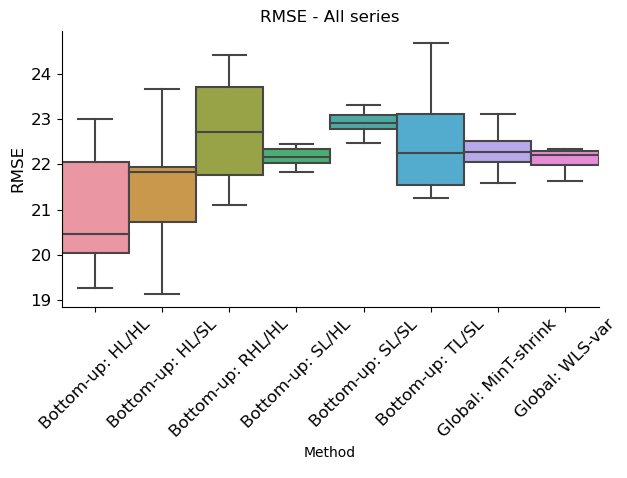
\includegraphics[width=\columnwidth]{assets/boxplot_rmse_allseries.png}}
    \caption{RMSE for all timeseries of the M5 dataset for a selected set of methods.}
    \label{fig:rmse_allseries}
  \end{figure}

  \begin{table}[t]
    \caption{Ablation experiment demonstrating the effect of sample subsampling and feature subsampling during tree-building on RMSE of all timeseries in the M5 dataset, in the \texttt{Bottom-up}-scenario. The base case refers to the optimal hyperparameters found by Optuna. For RMSE, lower is better, and bold indicates best method, with standard deviation in brackets.}
    \label{tab:samplingablation}
    \begin{center}
    {\small\setlength{\tabcolsep}{1pt} 
    \begin{tabular}{l c ccc}
    \toprule 
     &\multicolumn{3}{ c }{Hyperparameters}  \\
     \cmidrule(r){2-4}  
    Objective / Metric &\texttt{feature\_frac} &\texttt{bagging\_frac} &\texttt{bagging\_freq} &RMSE \\
    \toprule
    HL / HL \\
    \hspace{0.1cm} Base case &0.473 &0.999 &4 &20.9 (1.29) \\
    \hspace{0.1cm} No feature subsampling &1.0 &0.999 &4 &\textbf{20.5 (0.56)} \\
    \hspace{0.1cm} Mild feature subsampling &0.6 &0.999 &4 &21.5 (2.10) \\
    \hspace{0.1cm} No sample subsampling &0.473 &1.0 &n.a. &20.7 (1.13)  \\
    \midrule
    HL / SL &0.500 &0.673 &2 &21.4 (1.30) \\
    SL / HL &0.662 &0.987 &6 &22.2 (0.22) \\
    SL / SL &0.586 &0.933 &4 &22.9 (0.24) \\
  \bottomrule
  \end{tabular}}
  \end{center}
  \end{table}

  \paragraph{Analysis: time complexity} We investigate the computational time complexity required to perform training and prediction for each scenario and present the results in Table~\ref{tab:complexity}. The training and prediction time complexity is indicated by how respectively the training time and prediction time scales with respect to the default LightGBM training and prediction time complexity. First, we note that adding our hierarchical loss objective adds a component to the time complexity that scales with \(n^3\), as we need to compute \eqref{eq:hfp_grad}. However, our sparse implementation of the hierarchical loss reduces this component from \(n^3\) to \(n^2l\), effectively reducing the scaling from cubic to quadratic in the number of bottom-level timeseries, as \(l\) is generally small. In the reconciliation scenarios, we always need to compute a matrix inversion to solve \eqref{eq:p1} that scales cubically with the number of aggregations \(m^*\) or with the total number of timeseries \(m\). The first is not problematic as generally \(m^* \ll n\) in large-scale settings, but methods with this time complexity consequently trade in performance as we observed in Table~\ref{tab:allstores_rel}. To empirically verify the time complexity, we recorded the training and prediction time for each scenario. We show timings for training and prediction for a single store of the M5 dataset (4M training samples) and for entire M5 dataset (52M training samples), to provide an indication of scaling when the problem size increases by an order of magnitude. First, we note that using our sparse implementation of the HL reduces training time from respectively \(14.4x\) to \(1.3x\) for a single store and from \(8.5x\) to \(2.3x\) for all stores as compared to the baseline. Second, our sparse HL has a prediction time similar to the baseline (respectively 0.7x and 1.4x for making predictions for a single store or for all stores). Finally, we see that \textit{MinT-shrink} and \textit{ERM} require a similar training time when training for all stores, however the prediction time using our sparse HL is significantly lower. [As ML cost in production systems mainly consists of prediction costs, having a lower prediction time is beneficial[reference].] 
  \begin{table*}[t]
    \caption{Computational time complexity and observed relative timings for all scenarios. Timings are relative to the baseline (in italic). The complexity is indicated by how respectively the training time and prediction time scales with respect to the default LightGBM training/prediction time \(T\), where \(s\) denotes the number of samples per timeseries, \(n\) denotes the number of bottom-level time series in the hierarchy, \(n_l\) the number of time series in each level in the hierarchy and \(l\) the number of levels in the hierarchy, \(m\) the total number of time series, and \(m^{*} = m - n\).}
    \label{tab:complexity}
    \begin{center}
    {\small\setlength{\tabcolsep}{1pt} 
    \begin{tabular}{l c ccccccc}
    \toprule 
     &  &\multicolumn{2}{ c }{Complexity}   &\multicolumn{2}{ c }{Training time (s)} &\multicolumn{2}{ c }{Prediction time (s)}  \\
     \cmidrule(r){3-4} \cmidrule(r){5-6} \cmidrule(r){7-8} 
    Scenario/Objective  & Reconciliation &Training	&Prediction	&1 store &All stores &1 store &All stores \\
    \midrule																	
    \texttt{Bottom-up}																	\\
    \hspace{0.1cm} 	SL (dense)	&None & $O(T(s_nn))$	&$O(T(s_nn) + s_nn^3)$ &\textit{1.0}	&\textit{1.0}	&\textit{1.0}	&\textit{1.0}    \\
    \hspace{0.1cm} 	SL (sparse)	&None & $O(T(s_nn))$	&$O(T(s_nn) + s_nn^2l)$ &1.0	&1.0	&1.0	&0.8    \\
    \hspace{0.1cm} 	HL (dense)	&None & $O(T(s_nn + s_nn^3))$	 &$O(T(s_nn) + s_nn^3)$ &14.4	&8.5	&0.7	&1.7 \\
    \hspace{0.1cm} 	HL (sparse)	&None & $O(T(s_nn + s_nn^2l))$	 &$O(T(s_nn) + s_nn^2l)$ &1.3	&2.3	&0.7	&1.4 \\
    \midrule																	
    \texttt{Sep. agg.}																	\\
    \hspace{0.1cm} 	SL	&Base & $O(l \cdot T(s_ln_l))$	&$O(l \cdot T(s_ln_l))$	&1.2 &0.5	&0.3	&0.2    \\
    \hspace{0.1cm} 	SL	&OLS	& $O(l \cdot T(s_ln_l))$	&$O(l \cdot T(s_ln_l) + m^{*3})$ &1.2	&0.5	&0.3	&0.8		\\
    \hspace{0.1cm} 	SL	&WLS-struct	& $O(l \cdot T(s_ln_l))$	&$O(l \cdot T(s_ln_l) + m^{*3})$ &1.2	&0.5	&0.3	&0.8    \\
    \hspace{0.1cm} 	SL	&WLS-var	& $O(l \cdot T(s_ln_l))$	&$O(l \cdot T_p(n_l) + m^{*3})$ &1.2	&0.5	&0.3	&0.8    \\
    \hspace{0.1cm} 	SL	&MinT-shrink & $O(l \cdot T(s_ln_l))$	&$O(l \cdot T(s_ln_l) + m^3)$	&1.2	&0.5	&0.3	&6.0    \\
    \hspace{0.1cm} 	SL	&ERM & $O(l \cdot T(n_l))$	&$O(l \cdot T(s_ln_l) + m^3)$ &1.2	&0.5	&0.4	&2.0    \\
    \midrule																	
    \texttt{Global}																	\\
    \hspace{0.1cm} 	SL	&Base & $O(T(s_mm))$	&$O(T(s_mm))$	&4.2	&2.0	&3.3	&1.8    \\
    \hspace{0.1cm} 	SL	&OLS	& $O(T(s_mm))$	&$O(T(s_mm) + m^{*3})$	&4.2	&2.0	&3.3	&2.5    \\
    \hspace{0.1cm} 	SL	&WLS-struct	& $O(T(s_mm))$	&$O(T(s_mm) + m^{*3})$	&4.2	&2.0	&3.3	&2.5    \\
    \hspace{0.1cm} 	SL	&WLS-var	& $O(T(s_mm))$	&$O(T(s_mm) + m^{*3})$	&4.2	&2.0	&3.3	&2.5    \\
    \hspace{0.1cm} 	SL	&MinT-shrink & $O(T(s_mm))$	&$O(T(s_mm) + m^3)$	&4.2	&2.0	&3.4	&7.8    \\
    \hspace{0.1cm} 	SL	&ERM & $O(T(s_mm))$	&$O(T(s_mm) + m^3)$ &4.2	&2.0	&3.4	&4.1    \\
    \bottomrule
    \end{tabular}}
    \end{center}
    \end{table*}
  
  \subsection{Proprietary datasets} \label{subsec:proprietarydatasets}
  At bol.com, a LightGBM-based forecasting model is used as the primary product forecasting model. The model is used to forecast weekly product demand for 12 weeks. Every day, 12 separate models are trained, each tasked to forecast demand for a single week for every product. The model is used to forecast the majority of the products on sale at any moment, which are approximately 5 million unique items. We investigate the use of our sparse hierarchical loss function as a drop-in replacement for the existing Tweedie loss that is used within the company. The offline dataset consists of 38M training samples from the period January 2017 to the end of June 2021. We test on samples from the period July 2021 to January 2022. The baseline model for every weekly forecast model is a LightGBM model with a \textit{Tweedie Loss} (TL). The baseline model uses 19 proprietary features. 
  
  \paragraph{Experimental setup} We replace the TL with our HL and investigate forecasting performance on the test set. For the HL, we use the proprietary aggregations \textit{category} and \textit{subcategory}, each containing respectively [x] and [y] unique values. Thus, we have \(n = [x]\) bottom-level timeseries and \(m^* = [y]\) aggregated timeseries across \(l = 4\) levels: \textit{product} (bottom-level), \textit{category}, \textit{subcategory} and \textit{total}.

  \paragraph{Results} We present the results in Table~\ref{tab:bolresults}. On average, we find our sparse HL underperforms the existing TL model by about 5\%. We further investigate the performance by investigating how the RMSE varies across the 12 forecasting horizons Figure~\ref{fig:bol_rmse}. [This confirms the previous results + further deepdive + learnings] 

    \begin{table}[H]
    \caption{Forecast performance by RMSE of our offline test on bol.com data. Lower is better, bold indicates best method with standard deviation in brackets.}
    \label{tab:bolresults}
    \begin{center}
    \begin{tabular}{l c c}
    \toprule 
    &\multicolumn{2}{ c }{RMSE} \\
    \cmidrule(r){2-3}  \\
    Aggregation & TL & HL \\
    \midrule
    Product &2.0 () &2.1 () \\
    Subcategory &40 () &44 () \\
    Category &50 () &50 () \\
    Total &400 () &400 () \\
    \bottomrule
    \end{tabular}
    \end{center}
  \end{table}

  \begin{figure}[t]
    \centering
    \centerline{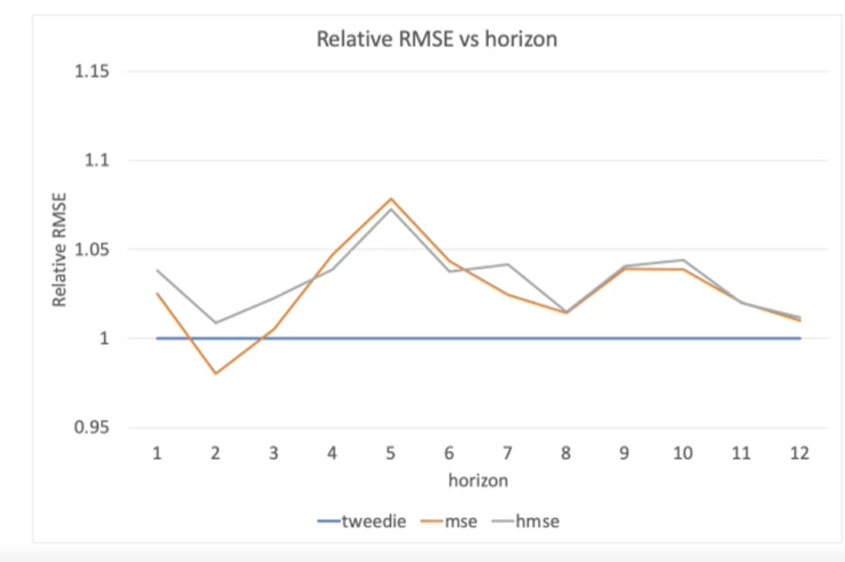
\includegraphics[width=\columnwidth]{assets/bol_rmse.png}}
    \caption{RMSE relative to the Tweedie baseline at product level for each forecasting horizon (week).}
    \label{fig:bol_rmse}
  \end{figure}

\section{Conclusion} \label{sec:conclusion}
  We introduced a sparse hierarchical loss function to perform hierarchical forecasting in large-scale settings. We demonstrated that we are able to outperform existing hierarchical forecasting methods both in terms of performance as measured by RMSE by up to 10\% as well as in terms of computational time required to perform the end-to-end hierarchical forecasting in large-scale settings, reducing prediction time as compared to the best hierarchical forecasting reconciliation method by a factor of 4. We empirically verified our sparse hierarchical loss in an offline test for bol.com, where we unfortunately could not verify the results from our offline test on public datasets. [additional learnings] 

  In addition to our main contributions, one of our main learnings has been that we could not find a benefit of having multiple models for separate aggregations in the hierarchy, as the bottom-up scenario we employed consistently outperformed other scenarios. This is in contrast with [ref, ref].

  For future work, we aim to extend our work to the setting of probabilistic forecasting by combining our sparse hierarchical loss with existing probabilistic forecasting frameworks from, e.g. \cite{sprangers_probabilistic_2021, hasson_probabilistic_2021, stankeviciute_conformal_2021}.


\section*{Acknowledgments}
  This research was (partially) funded by the Hybrid Intelligence Center, a 10-year program funded by the Dutch Ministry of Education, Culture and Science through the Netherlands Organisation for Scientific Research.\footnote{\url{https://www.hybrid-intelligence-centre.nl/}}

  All content represents the opinion of the authors, which is not necessarily shared or endorsed by their respective employers and/or sponsors.
  
  % We thank the reviewers for their constructive feedback and help on improving our work. 


\bibliographystyle{elsarticle-num-names} 
\bibliography{lib}

\clearpage

\appendix

\section{M5 Dataset} \label{app:m5dataset}
For each of the scenarios of our experiments in Section~\ref{sec:experiments}, we construct a set of features for the LightGBM model as given in Table~\ref{tab:features}. To facilitate the most `fair' comparison across methods, each model has the same features, and for the timeseries aggregations in the hierarchy we construct the features taken over the aggregation. 
\begin{table}
  \caption{Features used for the M5 dataset in our experiments.}
  \label{tab:features}
  \begin{center}
  {\small\setlength{\tabcolsep}{1pt} 
  \begin{tabular}{l l }
  \toprule 
  Feature & Description \\
  \midrule
  \texttt{Aggregation} & Aggregation level in the hierarchy \\
  \texttt{Value} & Identifier of timeseries of this aggregation \\   
  \texttt{sales\_lag1-7} & Lagged sales (target) (7 features) \\
  \texttt{sales\_lag28} & Sales 28 days ago \\ 
  \texttt{sales\_lag56} & Sales 56 days ago \\ 
  \texttt{sales\_lag364} & Sales last year \\ 
  \texttt{sales\_lag1\_mavg7} & Moving average of sales last 7 days \\
  \texttt{sales\_lag1\_mavg28} & Moving average of sales last 28 days \\ 
  \texttt{sales\_lag1\_mavg56} & Moving average of sales last 56 days\\ 
  \texttt{dayofweek} & Day of the week \\ 
  \texttt{dayofmonth} & Day of the month \\
  \texttt{weekofyear} & Week of year \\ 
  \texttt{monthofyear} & Month of year \\ 
  \texttt{sell\_price\_avg} & Sell price (average if aggregation)\\ 
  \texttt{sell\_price\_change} & Day-to-day change in sell price\\
  \texttt{weeks\_on\_sale\_avg} & Weeks on sale \\ 
  \texttt{snap\_CA} & State indicator for California \\ 
  \texttt{snap\_TX} & State indicator for Texas \\ 
  \texttt{snap\_WI} & State indicator for Wyoming \\
  \texttt{event\_type\_1\_enc} & Encoded events \\ 
  \texttt{event\_type\_2\_enc} & Encoded events \\
  \bottomrule
  \end{tabular}}
  \end{center}
\end{table}

\section{M5 model training \& optimization} \label{app:hyperparam}
We optimize the hyperparameters of our LightGBM models using Optuna \cite{akiba_optuna_2019}, using the settings found in Table~\ref{tab:hyperparams}. The validation is performed on a rolling-forward basis for 3 validation sets, where we use two years of data to predict the next 28 days ahead. After the hyperparameter optimization procedure, we use the average number of iterations at which the lowest validation loss was achieved across the 3 validation sets as the number of estimators to use in our final model.
\begin{table*}
  \caption{Key hyperparameters used in our experiments. The parameters with a search range included are optimized in a hyperparameter search.}
  \label{tab:hyperparams}
  \begin{center}
  {\small\setlength{\tabcolsep}{1pt} 
  \begin{tabular}{l l c c }
  \toprule 
  Parameter & Description & Default value & Search range \\
  \midrule
  \texttt{n\_estimators} & Number of trees in each model & 2000 & Lowest validation loss \\
  \texttt{n\_trials} & Number of optimization trials to run & 100 & \\  
  \texttt{learning\_rate} & Learning rate & 0.1 & \\  
  \texttt{n\_validation\_sets} & Number of validation sets & 3 & \\  
  \texttt{n\_days\_test} & Number of days in validation and test sets & 28 & \\
  \texttt{max\_levels\_random} & Max. number of levels when using a random hierarchy & 2 & \\  
  \texttt{\shortstack{max\_categories\_per \\ \_random\_level}} & Max. categories per level in the random hierarchy & 1000 & \\  
  \texttt{hier\_freq} & Frequency of performing the randomized hierarchical aggregation & 1 & \texttt{uniform($1$, $10$)}  \\  
  \texttt{lambda\_l1} & L1-regularization & 0 & \texttt{log\_uniform($10^{-8}$, $10^{1}$)} \\  
  \texttt{lambda\_l2} & L2-regularization & 0 & \texttt{log\_uniform($10^{-8}$, $10^{1}$)} \\  
  \texttt{num\_leaves} & Max. number of leaves per tree & 31 & \texttt{uniform($2^{3}$, $2^{10}$)} \\  
  \texttt{feature\_fraction} & Fraction of features to use to build a tree & 1.0 & \texttt{uniform($0.4$, $1.0$)} \\  
  \texttt{bagging\_fraction} & Fraction of training samples to use to build a tree & 1.0 & \texttt{uniform($0.4$, $1.0$)} \\  
  \texttt{bagging\_freq} & Frequency at which to create a new bagging batch & 1.0 & \texttt{uniform($1$, $7$)} \\  
  \texttt{min\_child\_samples} & Minimum number of samples per leaf & 20 & \texttt{log\_uniform($5$, $5000$)} \\  
  \bottomrule
  \end{tabular}}
  \end{center}
\end{table*}



\section{Experiments} \label{app:experiments}

\begin{sidewaystable*}[t]
  \caption{Forecasting results for all stores on the M5 dataset. We report mean RMSE scores across 10 random seeds with standard deviation in brackets. For the \texttt{Separate aggregations}-scenario, the results are based on 8 seeds, as 2 seeds produced erroneous results. Lower is better, and bold indicates best method for the aggregation, taking into account the standard deviation of the best method.}
  \label{tab:allstores_abs}
  \begin{center}
  {\small\setlength{\tabcolsep}{1pt} 
  \begin{tabular}{l c cccccccccccccc}
  \toprule 
   &&&& &  &\multicolumn{3}{ c }{Store}   &\multicolumn{2}{ c }{Product} &\multicolumn{3}{ c }{State} \\
   \cmidrule(r){7-9} \cmidrule(r){10-11} \cmidrule(r){12-14}
  Scen./Obj. & Metric  & Reconciliation &Product	&Department	&Category &Department	&Category	&Total &Store	&State &Department &Category &Total	&Total	&All series \\
  \midrule																	
  \texttt{Bottom-up}																	\\
  \hspace{0.1cm} 	SL	&SL	&None	&\textbf{1.94 (0.00)}	&568 (6.49)	&1116 (17.69)	&102 (0.58)	&197 (1.36)	&410 (2.93)	&6.67 (0.02)	&\textbf{3.67 (0.01)}	&256 (1.62)	&507 (4.26)	&1058 (9.88)	&\textbf{2350 (38.81)}	&22.9 (0.24)	\\
  \hspace{0.1cm} 	SL	&HL (ours)	&None	&\textbf{1.94 (0.00)}	&547 (6.70)	&\textbf{1076 (14.75)}	&99 (0.91)	&190 (2.19)	&396 (3.96)	&6.65 (0.01)	&3.67 (0.00)	&247 (2.14)	&489 (4.98)	&\textbf{1024 (8.29)}	&\textbf{2278 (32.61)}	&\textbf{22.2 (0.22)}	\\
  \hspace{0.1cm} 	HL (ours)	&HL (ours)	&None	&\textbf{1.94 (0.00)}	&\textbf{508 (28.48)}	&\textbf{985 (73.24)}	&\textbf{94 (1.64)}	&\textbf{179 (4.16)}	&\textbf{385 (13.21)}	&\textbf{6.58 (0.02)}	&\textbf{3.66 (0.01)}	&\textbf{229 (6.60)}	&\textbf{447 (16.94)}	&\textbf{974 (56.42)}	&\textbf{2203 (225.73)}	&\textbf{20.9 (1.29)}	\\
  \hspace{0.1cm} 	HL (ours)	&SL	&None	&1.95 (0.00)	&\textbf{516 (30.74)}	&\textbf{1008 (75.53)}	&97 (1.43)	&187 (3.38)	&400 (11.84)	&6.63 (0.03)	&\textbf{3.67 (0.01)}	&\textbf{236 (6.34)}	&\textbf{465 (15.19)}	&\textbf{1002 (54.04)}	&\textbf{2215 (243.47)}	&\textbf{21.4 (1.30)}	\\
  \hspace{0.1cm} 	TL	&HL (ours)	&None	&\textbf{1.94 (0.00)}	&553 (8.52)	&1102 (20.37)	&102 (0.64)	&197 (1.5)	&412 (3.46)	&6.68 (0.02)	&3.68 (0.00)	&252 (2.14)	&503 (5.2)	&1067 (13.51)	&\textbf{2407 (52.75)}	&22.9 (0.33)	\\
  \hspace{0.1cm} 	TL	&SL	&None	&1.95 (0.00)	&550 (31.99)	&\textbf{1067 (81.29)}	&104 (1.99)	&201 (5.13)	&417 (12.07)	&6.72 (0.03)	&3.7 (0.01)	&256 (7.93)	&506 (19.93)	&\textbf{1056 (49.08)}	&\textbf{2271 (197.35)}	&\textbf{22.6 (1.26)}	\\
  \hspace{0.1cm} 	TL	&TL	&None	&2.05 (0.00)	&979 (6.92)	&1908 (15.81)	&137 (0.61)	&269 (1.44)	&552 (3.5)	&8.44 (0.02)	&4.14 (0.01)	&379 (2.23)	&748 (5.07)	&1546 (13.72)	&3940 (43.2)	&36.0 (0.29)	\\
  \midrule																	
  \texttt{Sep. agg.}																	\\
  \hspace{0.1cm} 	SL	&SL	&Base	&1.96 (0.00)	&904 (23.27)	&1537 (54.5)	&117 (1.88)	&227 (3.81)	&681 (2.53)	&7.80 (0.03)	&3.76 (0.01)	&346 (6.92)	&1037 (8.9)	&1353 (35.64)	&3322 (125.61)	&33.9 (0.42)	\\
  \hspace{0.1cm} 	SL	&SL	&OLS	&1.98 (0.00)	&883 (14.82)	&1680 (36.14)	&132 (0.97)	&256 (2.22)	&520 (5.37)	&7.46 (0.02)	&3.87 (0.01)	&365 (3.97)	&732 (8.41)	&1396 (21.59)	&3079 (68.2)	&31.8 (0.46)	\\
  \hspace{0.1cm} 	SL	&SL	&WLS-struct	&1.96 (0.00)	&790 (8.45)	&1546 (17.33)	&117 (0.62)	&228 (1.12)	&457 (2.37)	&7.13 (0.01)	&3.79 (0.00)	&326 (2.71)	&650 (5.11)	&1308 (11.3)	&2992 (34.04)	&29.3 (0.26)	\\
  \hspace{0.1cm} 	SL	&SL	&WLS-var	&1.96 (0.00)	&719 (5.43)	&1404 (11.43)	&111 (0.35)	&216 (0.72)	&438 (1.48)	&7.08 (0.02)	&3.78 (0.01)	&299 (1.38)	&591 (2.65)	&1206 (6.41)	&2838 (26.78)	&27.1 (0.17)	\\
  \hspace{0.1cm} 	SL	&SL	&MinT-shrink	&1.96 (0.00)	&756 (15.00)	&1462 (29.92)	&111 (1.21)	&213 (2.49)	&422 (5.26)	&7.08 (0.04)	&3.78 (0.01)	&305 (4.51)	&597 (8.81)	&1193 (18.94)	&2879 (63.17)	&27.6 (0.49)	\\
  \hspace{0.1cm} 	SL	&SL	&ERM	&3.36 (0.03)	&883 (34.46)	&1739 (71.05)	&146 (1.81)	&262 (3.79)	&550 (8.43)	&13.33 (0.29)	&6.79 (0.10)	&367 (9.7)	&708 (22.6)	&1544 (41.54)	&3942 (132.91)	&35 (0.95)	\\
  \midrule																	
  \texttt{Global}																	\\
  \hspace{0.1cm} 	SL	&SL	&Base	&1.96 (0)	&699 (78.83)	&1468 (104.96)	&\textbf{94 (0.96)}	&183 (4.46)	&393 (11)	&6.68 (0.01)	&3.72 (0.00)	&254 (4.01)	&534 (13.97)	&1258 (90.54)	&4057 (220.21)	&30.0 (0.80)	\\
  \hspace{0.1cm} 	SL	&SL	&OLS	&1.96 (0)	&694 (29.29)	&1394 (49.44)	&106 (2.03)	&203 (3.93)	&438 (9.85)	&6.73 (0.01)	&3.71 (0.00)	&286 (8.94)	&572 (15.07)	&1266 (39.06)	&3149 (128.55)	&27.7 (0.75)	\\
  \hspace{0.1cm} 	SL	&SL	&WLS-struct	&1.95 (0)	&569 (8.08)	&1133 (18.36)	&97 (0.58)	&184 (1.69)	&383 (3.5)	&6.70 (0.01)	&3.70 (0.00)	&248 (2.39)	&492 (5.82)	&1047 (13.24)	&\textbf{2459 (44.76)}	&22.9 (0.29)	\\
  \hspace{0.1cm} 	SL	&SL	&WLS-var	&1.96 (0)	&552 (5.34)	&1084 (13.09)	&97 (0.66)	&185 (1.71)	&382 (3.47)	&6.78 (0.02)	&3.73 (0.01)	&245 (1.95)	&484 (4.71)	&\textbf{1014 (10.71)}	&\textbf{2309 (34.7)}	&\textbf{22.1 (0.23)}	\\
  \hspace{0.1cm} 	SL	&SL	&MinT-shrink	&1.95 (0)	&562 (11.06)	&1113 (27.8)	&\textbf{94 (1.16)}	&\textbf{178 (2.97)}	&\textbf{367 (5.94)}	&6.73 (0.02)	&3.71 (0.01)	&243 (3.74)	&479 (9.32)	&\textbf{1014 (18.79)}	&\textbf{2384 (61.06)}	&\textbf{22.3 (0.45)}	\\
  \hspace{0.1cm} 	SL	&SL	&ERM	&3.37 (0.02)	&722 (40.44)	&1453 (79.67)	&137 (3.82)	&249 (8.04)	&508 (21.61)	&13.56 (0.38)	&6.85 (0.08)	&332 (12.46)	&638 (22.86)	&1329 (56.91)	&3087 (154.87)	&29.7 (1.12)	\\ 
  
  \midrule
  \midrule
  \multicolumn{4}{l}{\texttt{Bottom-up}: \textit{impact of hierarchy}}																	\\
  \hspace{0.1cm} 	RHL (ours)	&HL (ours)	&None	&\textbf{1.94 (0.00)}	&560 (23.05)	&\textbf{1103 (62.42)}	&101 (1.10)	&194 (2.93)	&\textbf{407 (11.58)}	&6.69 (0.02)	&3.68 (0.01)	&252 (5.08)	&499 (13.51)	&\textbf{1053 (52.76)}	&\textbf{2352 (226.07)}	&\textbf{22.8 (1.17)}	\\
  \bottomrule
  
\end{tabular}}
  \end{center}
  \end{sidewaystable*}


\end{document}
\endinput
